% =========================================================================
% APPENDIX   [unlimited] --- everything that supports but would break the 8-page flow.
% Comes after \appendix in acl_latex.tex (sections renumber to A, B, C, ...).
% =========================================================================

\section{Full Per-Cell Results}
\label{sec:appendix-cells}
The primary artifact behind every number in the main text is the per-cell table
\texttt{composite\_cells.csv}, released with the code. Each row is one
\texttt{(model, dataset, condition)} cell and carries the three baseline-corrected
axes $(\Ppot,\Qual,\Sreason)$, the headline $\SFS$ and its two variants
($\SFS_{\text{prod}}$, $\SFS_{\text{covert}}$), and the raw diagnostics they are
computed from: the coherence-gated attack rate $\HAC$ (\texttt{raw\_hac}), the
coherence-retention rate (\texttt{clean\_rate}), the monitorability gap $\gapm$
(\texttt{gap}), and the safety-reasoning rate (\texttt{sr\_rate}). The grid contains
$5$ models $\times$ $2$ datasets $\times$ up to $11$ conditions; the $100$
non-baseline cells over the five models are the population summarised throughout
\S\ref{sec:compare}--\S\ref{sec:cot}.

Table~\ref{tab:appendix-model-family} gives the per-model, per-family mean $\SFS$
underlying the pooled ranking of Table~\ref{tab:intervention_family} and the
by-model view of Figure~\ref{fig:family-model}; it shows explicitly that the family
ordering is not uniform across models. A model-by-family rendering of the same
quantity is Figure~\ref{fig:appendix-heatmap}.

\begin{table}[t]
  \centering \small
  \setlength{\tabcolsep}{4pt}
  \begin{tabular}{@{}lcccc@{}}
    \toprule
    \textbf{Model} & Steer & Dir.\ abl. & SHIPS & Neuron \\
    \midrule
    \model{Qwen3-8B}       & 0.49 & \textbf{0.57} & 0.13 & 0.12 \\
    \model{Llama-3.1-8B}   & \textbf{0.88} & 0.58 & 0.30 & 0.51 \\
    \model{OLMo-3-think}   & \textbf{0.64} & 0.25 & 0.27 & 0.14 \\
    \bottomrule
  \end{tabular}
  \caption{Mean $\SFS$ by model and intervention family on the safety-trained tier
    (pooled over the two datasets; best family per model in bold). Steering is most
    faithful on \model{Llama-3.1} and \model{OLMo-3-think}; directional ablation wins
    on \model{Qwen3}. The two pre-alignment \model{OLMo-3-base} arms are controls and
    are reported separately (Table~\ref{tab:transfer}).}
  \label{tab:appendix-model-family}
\end{table}

\section{Judge Prompts and Validation}
\label{sec:appendix-judges}
Three LLM judges instrument the axes (\S\ref{sec:judges}):
\begin{itemize}[leftmargin=1.4em, itemsep=1pt, topsep=2pt]
  \item a \textbf{5-label safety + coherence judge} (Qwen3-30B) that classifies each
  final answer as refusal / safe-completion / harmful-completion and flags
  incoherent output; it feeds the coherence gate behind $\HAC$ (potency, $\Ppot$)
  and the coherence-retention rate (quality, $\Qual$);
  \item a \textbf{per-sentence safety-reasoning trace judge} and a \textbf{CoT-only
  predictor} (Qwen3-30B, vLLM backend): the trace judge marks which spans of a
  reasoning trace engage safety, and the CoT-only predictor estimates whether the
  final answer will be harmful \emph{from the reasoning trace alone}. The two
  together define the monitorability gap $\gapm=\mathrm{asr}_{\text{final}}-
  \mathrm{asr}_{\text{cot-pred}}$ behind $\Sreason$;
  \item a fine-tuned \textbf{12-label pathway judge} (Qwen3-14B, LoRA) that assigns
  the fine-grained pathway labels of Appendix~\ref{sec:appendix-pathway} to each
  parsed CoT prefix.
\end{itemize}
A metric is only standardizable if its instruments are reliable. The pathway judge
reaches $\kappa\approx0.96$ / $F_1\,0.98$ against a two-annotator human gold set,
where an un-tuned 30B baseline scores only $\kappa\,0.21$; the 5-label, CoT-only, and
trace judges are human-validated on the \texttt{batch\_v5\_002} annotation task. Two
auxiliary and three fine-grained labels reach only near-chance agreement and are
therefore excluded from every axis. The verbatim rubrics, the full per-label
$\kappa$ / $F_1$ tables, and the inter-annotator agreement are released with the
annotation tasks (\texttt{batch\_v5\_001}, \texttt{batch\_v5\_002}).

\section{Metric Definitions and Variants}
\label{sec:appendix-metric}
Each axis is mapped to $[0,1]$ and baseline-corrected against the same-%
\texttt{(model, dataset)} no-intervention cell $b$, with
$\clip(x)=\max(0,\min(1,x))$ (Eqs.~\ref{eq:pq}--\ref{eq:s}):
\[
\Ppot=\clip\!\Big[\tfrac{\HAC_c-\HAC_b}{1-\HAC_b}\Big],\quad
\Qual=\clip\!\Big[\tfrac{\mathrm{clean}_c}{\mathrm{clean}_b}\Big],
\]
\[
\Sreason=1-\clip\big[\,|\gapm_c|-|\gapm_b|\,\big].
\]
$\HAC$ (harmful-among-clean) is the attack-success rate over only those responses
that pass the coherence gate, so incoherent output cannot count as a successful
attack; $\mathrm{clean}$ is the coherence-retention rate; and $\gapm$ is the
monitorability gap. Potency is the fraction of the still-refusable headroom
$(1-\HAC_b)$ that the intervention converts into coherent harm.

The headline scalar is the geometric mean
$\SFS=(\Ppot\,\Qual\,\Sreason)^{1/3}$ (Eq.~\ref{eq:sfs}), which has a
``no-axis-left-behind'' property: any axis $\to0$ collapses the score. Two variants
appear in the diagnostics (Figure~\ref{fig:appendix-diagnostics}): the arithmetic
product $\SFS_{\text{prod}}=\Ppot\,\Qual\,\Sreason$, and the threat-oriented
$\SFS_{\text{covert}}=\Ppot\,\Qual\,(1-\Sreason)$, which rewards potent,
coherence-preserving harm whose danger is \emph{hidden} from the trace. Because
$1-\Sreason=\clip[\,|\gapm_c|-|\gapm_b|\,]$ uses the \emph{magnitude} of the gap,
$\SFS_{\text{covert}}$ also fires on strongly \emph{over}-warning cells (large
negative $\gapm$); the two cells that exceed $0.1$ in our grid are of exactly this
kind, not genuine covert failures (\S\ref{subsec:cot-monitor}). The primary object
we report is the $(\Ppot,\Qual,\Sreason)$ vector with a Pareto front
(Figure~\ref{fig:appendix-pareto}); the scalar is always reported \emph{with} the
vector, following the multi-metric precedent of HELM \citep{liang2023helm}.

\section{Additional Figures}
\label{sec:appendix-figs}
Figures~\ref{fig:appendix-heatmap}--\ref{fig:appendix-familydose} collect the
composite views that support the body but do not fit its flow: the model-by-family
$\SFS$ heatmap, the clean Pareto front per model, the metric-diagnostics panel
(including the raw-ASR vs.\ $\SFS$ ranking agreement), and the full 12-panel
family dose-response of which Figure~\ref{fig:dose-response} is the compact form.

\begin{figure}[t]
  \centering
  
\includegraphics[width=\columnwidth]{figures/composite_04_model_family_sfs_heatmap.png}
  \caption{Mean $\SFS$ by model and intervention family (numeric form in
    Table~\ref{tab:appendix-model-family}).}
  \label{fig:appendix-heatmap}
\end{figure}

\begin{figure}[t]
  \centering
  
\includegraphics[width=\columnwidth]{figures/composite_07_pareto_frontier_clean.png}
  \caption{Clean Pareto view of the composite metric: induced potency $\Ppot$ against
    retained selectivity $\Qual\Sreason$, per model, with iso-$\SFS$ contours.}
  \label{fig:appendix-pareto}
\end{figure}

\begin{figure}[t]
  \centering
  
\includegraphics[width=\columnwidth]{figures/composite_08_metric_diagnostics.png}
  \caption{Metric diagnostics. Raw $\HAC$ overstates the intervention effect (top
    left); $\SFS$ decomposes as potency times retained selectivity (top right);
    raw-ASR ranking agreement with $\SFS$ per model (bottom left); and the family
    ordering is robust to reasonable scalar variants (bottom right). The bottom-left
    $\tau$ pools both datasets per condition (min.\ $0.80$); the body's $\tau$ down to
    $0.73$ (\S\ref{subsec:c1}) instead ranks the dataset-averaged scores, which is the
    more conservative reading.}
  \label{fig:appendix-diagnostics}
\end{figure}

\begin{figure}[t]
  \centering
  
\includegraphics[width=\columnwidth]{figures/composite_09_family_dose_response.png}
  \caption{Full dose-response across intervention families (each of $\Ppot,\Qual,
    \Sreason,\SFS$ against the family's strength ladder), the expanded form of the
    compact Figure~\ref{fig:dose-response}.}
  \label{fig:appendix-familydose}
\end{figure}

\section{Pathway Taxonomy and Full Profile}
\label{sec:appendix-pathway}
The 12-label pathway judge (\S\ref{sec:judges}, Appendix~\ref{sec:appendix-judges})
tags each parsed CoT prefix with the fine-grained labels below, ordered along the
recognise\,$\to$\,refuse\,$\to$\,comply arc and grouped into the six stages used by
the radar axes:
\begin{enumerate}[leftmargin=1.4em, itemsep=0pt, topsep=2pt]
  \item \textbf{Recognition:} \texttt{risk\_acknowledgment}, \texttt{policy\_awareness}.
  \item \textbf{Intent assessment:} \texttt{intent\_assessment}.
  \item \textbf{Refusal initiation:} \texttt{refusal\_initiation},
        \texttt{refusal\_maintenance}.
  \item \textbf{Refusal suppression:} \texttt{refusal\_suppression}.
  \item \textbf{Rationalisation:} \texttt{benign\_motive\_invention},
        \texttt{educational\_framing}, \texttt{legal\_disclaimer\_laundering}.
  \item \textbf{Execution:} \texttt{task\_decomposition},
        \texttt{procedural\_planning}, \texttt{operational\_detail}.
\end{enumerate}
The compact five-stage view of Table~\ref{tab:cot-signature} pools recognition with
intent assessment and reports execution separately from operational detail.

Table~\ref{tab:appendix-pathway} gives the full 12-label rates for
\model{OLMo3-think} on JailbreakBench (rate over parsed CoT-prefixes, so the
population differs from the harmful-among-clean rows of
Table~\ref{tab:cot-signature}). Relative to the baseline, the localized families
(SHIPS, Neuron) and directional ablation barely perturb the profile, whereas the
strongest steering condition collapses recognition and refusal while lifting
procedural planning and operational detail---the dose-response of
Figure~\ref{fig:cot-dose}. Figure~\ref{fig:appendix-reasoning-radar} shows the
complementary cross-model view: the reasoning and non-reasoning classes trace
opposite shapes on the six grouped axes.

\begin{table}[t]
  \centering \scriptsize
  \setlength{\tabcolsep}{3pt}
  \resizebox{\columnwidth}{!}{%
  \begin{tabular}{@{}lccccc@{}}
    \toprule
    \textbf{Label} & base & steer\,$a1.5$ & abl. & SHIPS\,8 & Neur.\,1024 \\
    \midrule
    risk\_acknowledgment      & 0.29 & 0.03 & 0.26 & 0.26 & 0.29 \\
    policy\_awareness         & 0.25 & 0.02 & 0.23 & 0.28 & 0.28 \\
    intent\_assessment        & 0.17 & 0.21 & 0.15 & 0.15 & 0.17 \\
    refusal\_initiation       & 0.36 & 0.02 & 0.35 & 0.38 & 0.37 \\
    refusal\_maintenance      & 0.10 & 0.02 & 0.08 & 0.14 & 0.10 \\
    refusal\_suppression      & 0.01 & 0.07 & 0.01 & 0.01 & 0.01 \\
    benign\_motive\_invention & 0.06 & 0.01 & 0.05 & 0.04 & 0.06 \\
    educational\_framing      & 0.04 & 0.05 & 0.05 & 0.05 & 0.05 \\
    legal\_disc.\_laundering  & 0.04 & 0.02 & 0.04 & 0.05 & 0.04 \\
    task\_decomposition       & 0.13 & 0.07 & 0.13 & 0.17 & 0.14 \\
    procedural\_planning      & 0.18 & 0.46 & 0.21 & 0.17 & 0.16 \\
    operational\_detail       & 0.20 & 0.65 & 0.23 & 0.19 & 0.18 \\
    \bottomrule
  \end{tabular}}
  \caption{Full 12-label pathway rates for \model{OLMo3-think} on JailbreakBench
    (rate over parsed CoT-prefixes). Columns: baseline, strongest steering
    ($\alpha{=}1.5$), directional ablation, SHIPS top-8, Neuron top-1024. Only
    steering departs materially from the baseline profile.}
  \label{tab:appendix-pathway}
\end{table}

\begin{figure}[t]
  \centering
  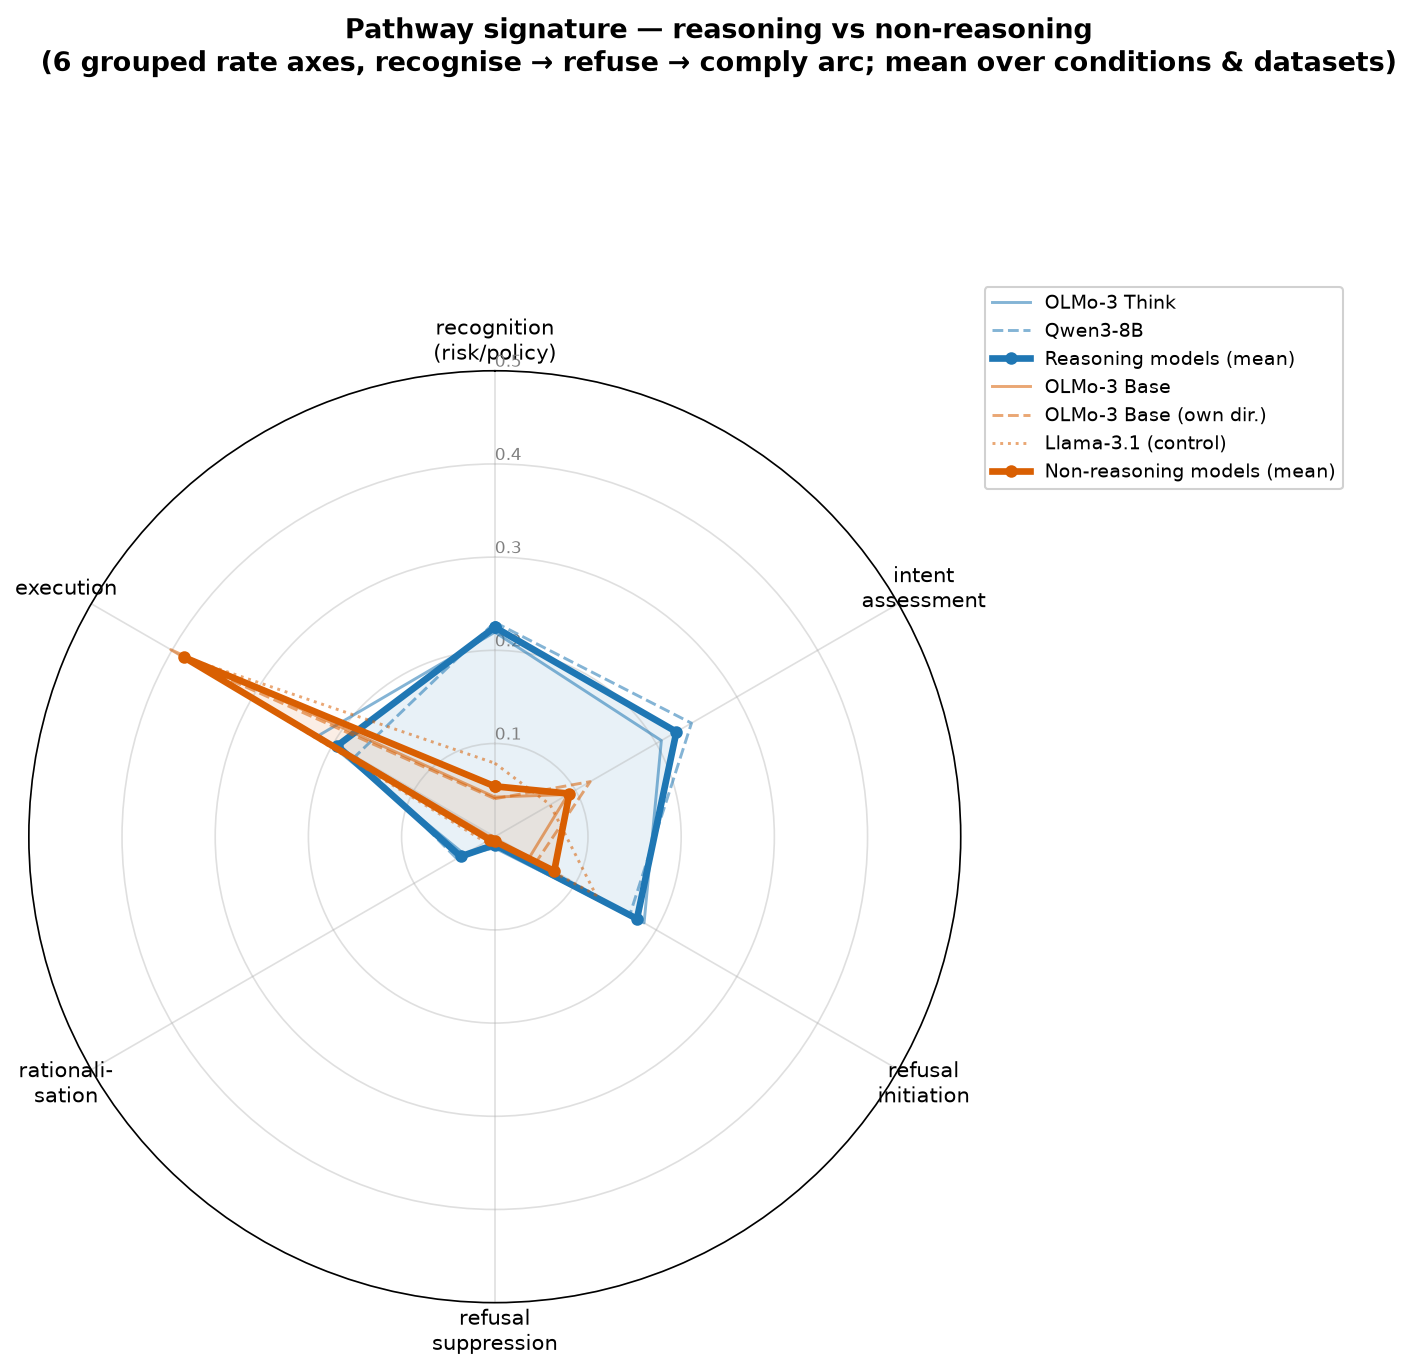
\includegraphics[width=\columnwidth]{figures/pathway_radar_reasoning.png}
  \caption{Pathway signature, reasoning vs non-reasoning models, on the six grouped
    axes (mean over conditions and datasets). The two classes trace opposite shapes:
    reasoning models keep recognition and refusal-initiation high and execution low;
    non-reasoning models do the reverse.}
  \label{fig:appendix-reasoning-radar}
\end{figure}
